\documentclass[10pt]{article}

\usepackage{graphicx}
\usepackage{float}

% paragraph spacing
\setlength{\parskip}{0.2em}

% section fontsize
\usepackage{sectsty}
\sectionfont{\fontsize{12}{15}\selectfont}

% margin
\usepackage{geometry}
\geometry{a4paper, portrait, margin=2cm}

% Set column width
\usepackage{array}
\newcolumntype{L}[1]{>{\raggedright\let\newline\\\arraybackslash\hspace{0pt}}m{#1}}
\newcolumntype{C}[1]{>{\centering\let\newline\\\arraybackslash\hspace{0pt}}m{#1}}
\newcolumntype{R}[1]{>{\raggedleft\let\newline\\\arraybackslash\hspace{0pt}}m{#1}}

\begin{document}
%%---------------------------------------
% Title
%---------------------------------------
\noindent
\begin{tabular}{lll R{8.0cm}}
\textbf{Members:} & \textbf{Taimoor Tariq}      & \textbf{20174577} & \textbf{Neural network EE538}\\
\textbf{}         & \textbf{Juan Luis Gonzalez} & \textbf{20178196} & \textbf{Project proposal}\\
\textbf{}         & \textbf{Thang Vu}           & \textbf{20174587} & \textbf{1/Nov/2017}
\end{tabular}\\
\rule[2ex]{\textwidth}{2pt}

%\vspace{0.5cm}
{\Large\centerline{\textbf{Video Super-Resolution Using Convolutional Neural Networks}}}

%%----------------------------------------
% Content
%%----------------------------------------
\section{Goal} % (fold)
\label{sec:goal}
Video Super Resolution (VSR) has remained a challenging problem although some improvement is obtained in recent years. In this project, our goal to design an improved algorithm and network architecture to address this problem. Our model will be compared to the current state-of-the-art, and it is expected that we will obtain better accuracy. 
% section goal (end)

\section{Background} % (fold)
\label{sec:background}
Super Resolution (SR) is the enhancement of image/video resolution. Although SR is a classical problem, it is inherently ill-posed as there are many possibilities to recover for a given low-resolution frame. Typically, SR algorithms can be divided roughly into two categories, which are model-based and learning-based algorithms. Model-based algorithms such as Baysesian approaches have been used for a long time, but with the advent of Deep Learning and Convolutional Neural Networks (CNN), there is great potential for learning-based approaches for image/video super resolution.

Image super resolution using CNN has been a topic of a great amount of research in recent years. In theory, CNN is able to learning a non-linear mapping from input to output, producing high-resolution mappings of low-resolution input \cite{dong2016image}. Some methods use input images of smaller sizes and learn mappings to high resolution, whereas other techniques first make use of bicubic interpolation to scale the image then use CNN to improve resolution \cite{dong2016image}. SRCNN is the first model that prove the efficiency of CNN in recovering resolution for single image \cite{dong2016image}. 

\begin{figure}[H]
    \centering
    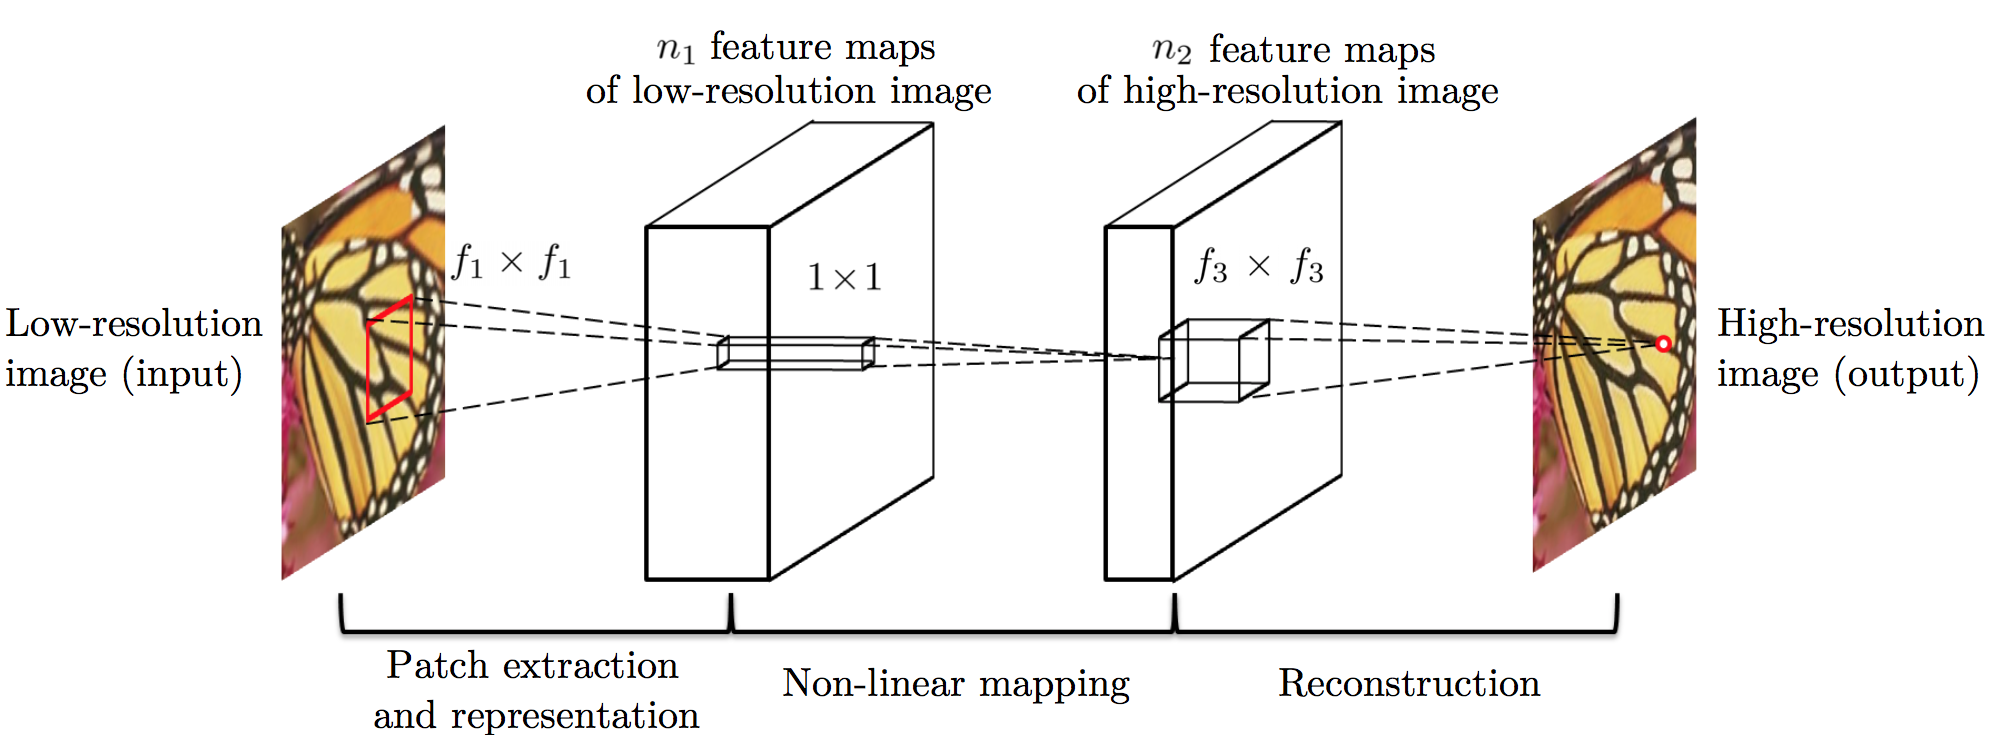
\includegraphics[scale=0.4]{figs/cnn.png}
    \caption{fadsf}
    \label{fig:1}
\end{figure}


% section background (end)


\bibliographystyle{IEEEtran}
\bibliography{refs}
\end{document}
